%%%%%%%%%%%%%%%%%%%%% PREAMBLE %%%%%%%%%%%%%%%%%%%%%
\documentclass{beamer}

% include frame number on each frame
\setbeamertemplate{footline}{\quad \insertframenumber/\inserttotalframenumber}
%%%%%%%%%%%%%%%%%%%%% DOCUMENT %%%%%%%%%%%%%%%%%%%%%
\begin{document}
\title{Information Theoretic Dependence Estimators for Time Series}
\author[Singh]{Shashank Singh}
\date{April 30, 2015}
\institute{Carnegie Mellon University\\10-704 Spring '15}
% \frame{\titlepage}

\frame{\frametitle{Nonparametric Dependence Estimators for Time Series}
  \begin{itemize}
    \item recall that we use mutual information to test independence
    \item quantities for IID data don't work for time series
    \begin{itemize}
      \item want to test $\{X_i\}_{i = 1}^n \perp \{Y_i\}_{i = 1}^n$
            rather than $X \perp Y$
      \item mutual information decays with lag effects
        \begin{figure}[h!]
          \centering
          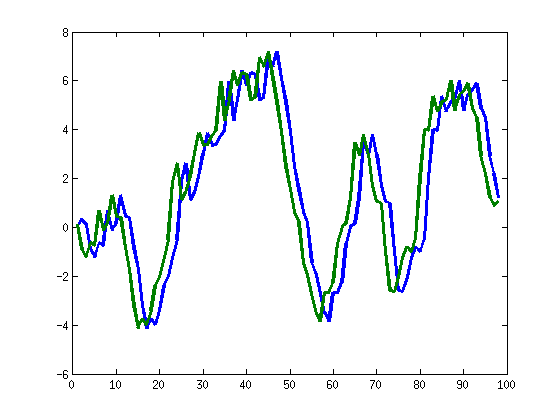
\includegraphics[width=0.5\textwidth]{ts}
        \end{figure}
    \end{itemize}
  \end{itemize}
}

\frame{\frametitle{Transfer Entropy and Mutual Information Rate}
  For time series that are $\beta$-Markov and stationary, we can use:
  \begin{itemize}
    \item Transfer entropy - additional predictive power of $X$ on $Y$:
    \begin{align*}
      T_{X \to Y}
       &  = H(Y_n | \{Y_i\}_{i = n - \beta}^{n - 1})
          - H(Y_n | \{(X_i,Y_i)\}_{i = n - \beta}^{n - 1}) \\
       &  = I(Y_n; \{X_i\}_{i = n - \beta}^{n - 1} | \{Y_i\}_{i = n - \beta}^{n - 1})
    \end{align*}
    \item Mutual Information Rate - average information shared
\begin{align*}
I_R(X;Y)
 &  = \lim_{n \to \infty}
        \frac{I(\{X_i\}_{i = n - \beta}^n,\{Y_i\}_{i = n - \beta}^n)}{n}    \\
 &  = T_{Y \to X} + T_{X \to Y} + I(X_n;Y_n | \{(X_i,Y_i)\}_{i = n - \beta}^n)
\end{align*}
  \end{itemize}
}

\frame{\frametitle{Experimental Results}
  \begin{itemize}
    \item power of permutation tests for independence:
  \end{itemize}
  \vspace{-10mm}
  \begin{columns}
    \begin{column}{0.33\textwidth}
      \begin{center}
        \begin{figure}[h!]
          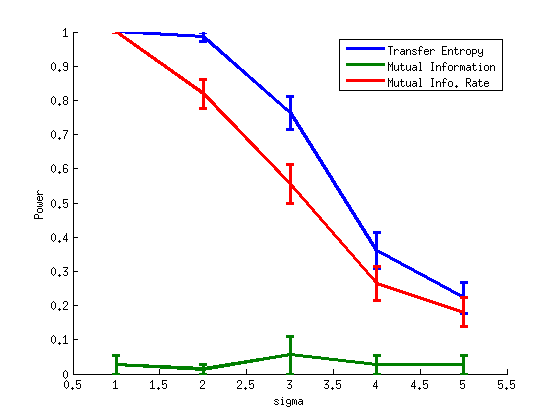
\includegraphics[width=1.3\textwidth]{TE_sim}
        \end{figure}
        $X_i = \epsilon_i$\\
        $Y_{i + 1} = X_i + \delta_i$
      \end{center}
    \end{column}
    \begin{column}{0.33\textwidth}
      \begin{center}
        \begin{figure}[h!]
          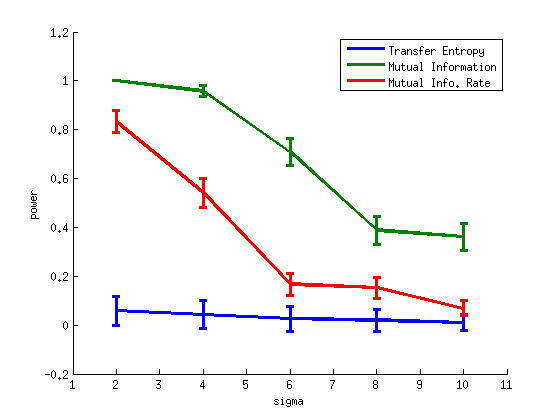
\includegraphics[width=1.3\textwidth]{MI_sim}
        \end{figure}
        $X_{i + 1} = X_i + \epsilon_i$\\
        $Y_{i + 1} = X_{i + 1} + \delta_i$
      \end{center}
    \end{column}
    \begin{column}{0.33\textwidth}
      \begin{center}
        \begin{figure}[h!]
          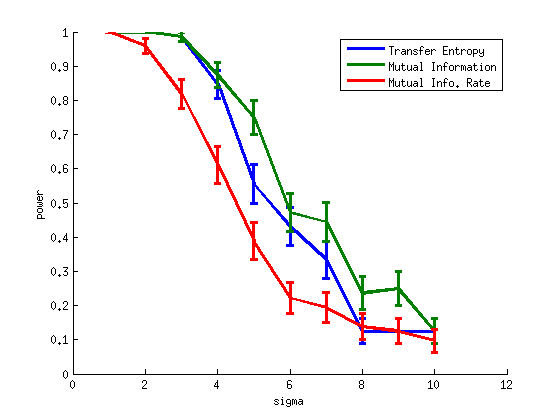
\includegraphics[width=1.3\textwidth]{all_sim}
        \end{figure}
        $X_{i + 1} = X_i + \epsilon_i$\\
        $Y_{i + 1} = X_i + \delta_i$
      \end{center}
    \end{column}
  \end{columns}
  \vspace{5mm}
  \begin{itemize}
    \item mutual information rate can be safest, but has lower power
  \end{itemize}
}
\end{document}
